\documentclass[12pt,letterpaper]{article}
\usepackage{mla}
\begin{document}
\begin{mla}{Paul}{English}{ENG 2010-002}{Professor Argyle}{\today}{Position / Proposal}
Every day we drive around in cars that are equipped with air conditioning, and heated seats. Cars that have 8+ cylinder engines, oversized tires, or racing modifications. Cars that have seats for passengers that we rarely fill, and truck beds for loads that are rarely hauled. Every day we use mobile phones and laptops with batteries that stay charged for hours. Devices, batteries, and subtle conveniences that were built in large factories. Factories that release excess amounts of harmful materials and pollutants into the atmosphere throughout the year. Every day we heat and cool our living spaces and our offices using filtered clean air. We move air around, and we leave the thermostats set to general temperatures. Lights are run in these buildings during the day, and sometimes even at night. All this energy is being supplied largely by fossil fuels, and natural resources.

Individually we end up spending very little time thinking about the environment outside. Instead, we enjoy our comforts, we work, we focus on family, and in general we keep ourselves busy. Why would we spend the time to worry about the environment? A lackadaisical attitude towards the environment can cause us to ignore the some of these issues, allowing people and corporations with financial goals to discredit the valid science behind global warming, and we end up slow to action when we need change the most.

\section{Errors \& Calculation Bias in Climate Data}
Scientific validity hinges on the evidence used as the foundation of any discovery, experiment, or observation. We have gathered evidence confirming a growing temperature trend in our global atmosphere. If this data isn't what we expect then a lot of the hypotheses and conclusions we've heard about global warming must be false. Skeptics of climate change have a goal in discrediting this research and analysis, in order to strengthen their position.

Skeptics of the global warming data often cite differences in GISTEMP data compared to similar Satellite records. The Urban Heat Island effect, UHI, warmer anomaly invalidly represented due to populous areas, is sometimes offered as a reason why aggregated temperature data may be warmer than it should be. There are also arguments saying that there are too many errors in individual temperature readings, labeled as micro-site bias. Some data skeptics attack the organization, or the GISTEMP project lead, James Hansen, in an attempt to discredit authority (``Correcting GISTEMP"). When combining these steps an opposing viewpoint can be fabricated. Using and changing data in this way doesn't always follow logical reasoning. Dramatic differences can be seen when comparing an invalid temperature analysis, fig. 1.0, where data has been changed to show a less dramatic curve, to a normal analysis, fig. 1.1 (``Correcting GISTEMP"). This difference can be used to strengthen a climate skeptics position, knowing that most readers lack the understanding or time to determine the validity of these analysis changes

\begin{center} % Figures
\begin{picture}(320,235)
\put(0,0){
\setlength{\fboxsep}{20pt}
\setlength{\fboxrule}{1pt}
\fbox{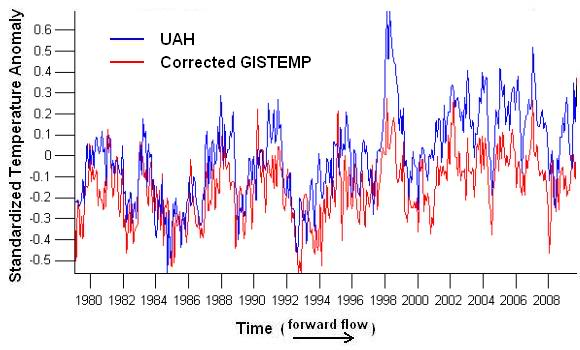
\includegraphics[scale=0.5]{invalid-corrected-gistemp.jpeg}}
}
\put(15,-15){Figure 1.0: UAH Satellite record vs. skewed GISTEMP readings (``Correcting GISTEMP").}
\end{picture}
\end{center}
\vspace{15 mm}

\begin{center} % Figures
\begin{picture}(320,235)
\put(0,0){
\setlength{\fboxsep}{20pt}
\setlength{\fboxrule}{1pt}
\fbox{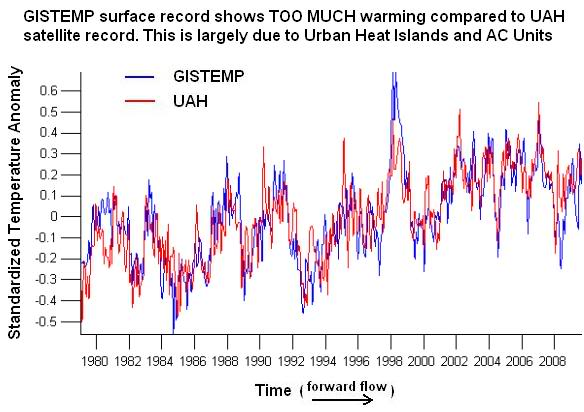
\includegraphics[scale=0.5]{initial-uah-gistemp.jpeg}}
}
\put(15,-15){Figure 1.1: UAH Satellite record vs. original GISTEMP readings (``Correcting GISTEMP").}
\end{picture}
\end{center}
\vspace{15 mm}

Many of these arguments relating to data are often lacking professional citations, contain logical fallacies, or are misguided. It's true that when compared GISTEMP data is different from UAH Satellite records, however sensor data is expected to be different, and there is no evidence citing statistically significant variations in the two records. Pertaining to UHI, the GISTEMP study and other studies do their best to compensate for urban warm spots by averaging anomaly differences across neighboring regions (``GISTEMP"). Micro-site bias is also a valid issue, however misreading of individual station data is often discovered as an outlier in the data set, and can be safely removed from final analysis. Attempts to discredit the organization or researchers tend to follow straw man arguments, a logical fallacy that misrepresents the opponents position.

Many of the same arguments used against the GISTEMP study can be found trying to oppose other data sets like the UAH satellite temperature dataset, the RSS MSU, the HadCRUT3, the NCDC absolute, the NCDC anomaly, the CET, or the SIDC, which are all differing surface temperature studies.

\section{Some Skeptics Accept Warming, But Argue Against Human Causes}
When arguing about climate change, some opponents will accept that temperatures have been increasing, or that global warming is happening, but they will deny that humans are a significant factor in causing the problem. Blame is shifted to natural or external causes that have been and will always be outside of our control.

Evidence for human impact on the environment can be shown in several ways. The typical method of showing human influence revolves around our CO2 and greenhouse gas emissions. The Carbon Dioxide Information Analysis Center, CDIAC, an office of the U.S. Department of Energy, estimates that we deposited upwards of 32 billion metric tons of carbon dioxide units into the atmosphere in the year 2008. (Boden). Additionally, we have ice core data that shows clear incrementing trends of CO2 averages (Inderm\"{u}hle). The CO2 measurements found in the air at the Mauna Loa observatory in Hawaii show similar trends of growth in CO2 levels (Tans). With evident growing levels of CO2, we hypothesize that radiation and energy will exit our atmospheric system at lower rates than in a system with less CO2. Our observations match this hypothesis, correctly showing that higher CO2 levels in our environment cause radiation to remain longer in our atmosphere. (Harries) (Chen). This means that we have valid evidence of post-industrial humans significantly contributing to CO2 levels in the atomsphere, this CO2 remains in the atmosphere collecting radiation that might normally escape, and this radiation can be linked as a cause of the warming we are seeing in our observed surface temperature data.

\section{The Politics Of Global Warming}
In addition to data skeptics, and those who deny our impact in the environment are organizations and companies whose short term interests do not coincide with decreasing the use of fossil fuels. Fossil fuels are one of the leading causes of increased greenhouse gasses (CDIAC).
In 2011 spending for oil and gas related lobbying exceeded \$149 million dollars, and included contributors like Conoco Phillips, Shell, Exxon Mobil, Chevron, and the American Petroleum Institute. Yearly contributions, excluding incomplete data from 2012, show a clear trend of ever increased spending to lobby for the oil and gas industry (U.S. Office of Public Records Fig. 2).

\begin{center} % Figures
\begin{picture}(320,235)
\put(0,0){
\setlength{\fboxsep}{20pt}
\setlength{\fboxrule}{1pt}
\fbox{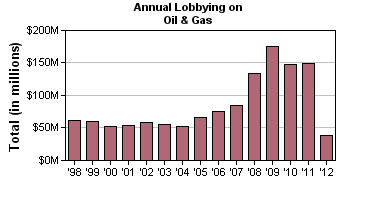
\includegraphics[scale=0.6]{oil-and-gas-lobbying-2012.png}}
}
\put(15,-15){Figure 2.0: Oil \& gas lobbying in the United States (U.S. Office of Public Records).}
\end{picture}
\end{center}
\vspace{15 mm}

Though Exxon Mobil has never officially denied global warming, evidence has been shown that they have tried to discredit and add uncertainty to climate studies (``Smoke, Mirrors, \& Hot Air"). This and companies that are similar have created road blocks of legislation towards improving the environment, and they have sought out short term financial gain without considering the long term cost of a degraded environment. They have profited off government subsidies, and are able to make a very large negative impact.

Surprisingly, not all of these corporations take a negative stance towards a cleaner environment. Exxon Mobil has released more recent updates showing their to support for climate science and interest in helping (Mufson). Other large oil companies wanting to help develop clean energy sources, and nuclear energy organizations have long sought out the elimination of fossil fuel usage.

\section{Understanding What We Can Do}

The arguments against improving the environment and cutting fossil fuel consumption don't withstand critical peer review. When we understand that we're dealing with a real problem we can better set up goals and drive our society towards positive change. Our society is made up of individuals, all contributing and sharing, and even though we can't always compete directly with the heavy financial interests and misinformation regarding climate degradation, we can improve our own impact. Knowing that the main causes of CO2 and increased green house gasses in our environment come from the consumption of fossil fuels helps us pinpoint areas where we can improve the most.

\subsection{Vehicles}
We've become a commuter society, building vast transport infrastructure and making cars easy to purchase using convenient loan systems. Commuting daily takes it's toll on the environment. Commuters in the United States alone are shown to release significant amounts of pollutants into the atmosphere every year. There are many things we can do to cut down on driving. We can organize car-pools and ride-sharing that makes each vehicle more efficient by spreading the cost amongst a few. We can schedule telecommute days into our schedule where we can avoid driving and transportation altogether, relying on the speed and efficiency of communications over the internet. We can use public transportation more often. We can relocate to a closer proximity and walk or bike as a commute. We can buy efficient engines that recycle braking energy to conserve fuel. We can even push for robotic technology that will enable car sharing and computer controlled fuel efficiencies of our current vehicles. We can avoid vanity travel and airplane flights in favor more efficient methods of vacation. Our transportation infrastructure does not have to disappear and we don't need to cut ourselves off from each other, we just need moderation. We must to choose lifestyles that don't required to travel and long distances.

\subsection{Households}
Amongst our homes there are many things we can change to improve sustainability. Installing specialized solar cells can provide both energy, and heating in a self-sufficient manner. Small wind turbines can generate power in windy clear areas. We can even receive tax and utility credits by using these alternative energy sources. Our food consumption can improve by finding local farms who don't need to ship their produce and goods long distances, an unsustainable practice. Planting our own gardens and composting trash is cheap and efficient, requiring only time and effort to achieve. Avoiding the newest gadgets, and battery powered toys also helps to prevent expensive consumption, and polluting production of these devices.

\subsection{Speaking Up}
For every step we take to improve our individual carbon footprints, we must also share our knowledge and help others in part. Our climate problems were not created by uniquely identifiable offenders, but by groups of society over time. Likewise the solution does not lie in herculean efforts, but in cooperative and grassroots based teamwork. We must work together to dismiss the fallacies and misunderstandings that create opposition. Educating those around us on sustainable practices. We should always speak up to our leaders and elected representatives, so that they can understand our interest in protecting the environment.

\section{Conclusion}
There is no quick fix to solving climate issues. What we have ahead of us is an uphill battle, which will require work on multiple fronts. We must discourage reckless behavior relating to the environment, and create new methods of thinking. By understanding what it is we are doing to damage the environment we can restrict these behaviors. By improving our acceptance of these facts we help to promote the larger problems our society faces. With effort many of us can lower our footprints in the environment, cooperatively leading to a positive impact at global scale.

\begin{workscited}

\bibent
Boden, T.A., G. Marland, and R.J. Andres. 2010. \textit{Global, Regional, and National Fossil-Fuel CO2 Emissions.} Carbon Dioxide Information Analysis Center, Oak Ridge National Laboratory, U.S. Department of Energy, Oak Ridge, Tenn., U.S.A. doi 10.3334/CDIAC/00001\_V2010

\bibent
Chen, Claudine, John Harries, Helen Brindley, and Mark Ringer. ``Spectral Signatures of Climate Change in the Earth�s Infrared Spectrum between 1970 and 2006." \textit{EUMETSAT}. 2007. Web. 05 July 2012. $<$http://www.eumetsat.int/Home/Main/AboutEUMETSAT/Publications/ConferenceandWorkshopProceedings/2007/groups/cps/documents/document/pdf\_conf\_p50\_s9\_01\_harries\_v.pdf$>$.

\bibent
``Correcting GISTEMP." Web log post. Denial Depot. N.p., 8 Sept. 2009. Web. 05 July 2012. $<$http://denialdepot.blogspot.com/2009/11/correcting-gistemp.html$>$.

\bibent
Harries, John E., Helen E. Brindley, Pretty J. Sagoo, and Richard J. Bantges. ``Increases in Greenhouse Forcing Inferred from the Outgoing Longwave Radiation Spectra of the Earth in 1970 and 1997." \textit{Nature} 410 (2001): 355-57. Print.

\bibent
Inderm\"{u}hle A., Et. Al. 2008. \textit{Holocene carbon-cycle dynamics based on CO2 trapped in ice at Taylor Dome, Antarctica.} Nature 398:121-126.

\bibent
Mufson, Steven. ``Exxon Mobil Warming Up To Global Climate Issue." \textit{The Washington Post} 10 Feb. 2007: n. pag. 9 Feb. 2007. Web. 5 July 2012. $<$http://www.washingtonpost.com/wp-dyn/content/article/2007/02/09/AR2007020902081.html$>$.

\bibent
"Smoke, Mirrors, \& Hot Air." \textit{Union Of Concerned Scientists} (2007): Union Of Concerned Scientists. Jan. 2007. Web. 05 July 2012. $<$http://www.ucsusa.org/assets/documents/global\_warming/exxon\_report.pdf$>$.

\bibent
United States. Department of Commerce. National Oceanic \& Atmospheric Administration. \textit{Trends in Atmospheric Carbon Dioxide.} By Peter Tans and Ralph Keeling. N.p., n.d. Web. 05 July 2012. $<$http://www.esrl.noaa.gov/gmd/ccgg/trends/$>$.

\bibent
United States. Senate. Office of Public Records. \textit{Contributions Reporting.} Web. 05 July 2012. $<$http://www.senate.gov/pagelayout/legislative/g\_three\_sections\_with\_teasers/lobbyingdisc.htm$>$.

\end{workscited}
\end{mla}
\end{document}
